% dynamic execution-time hardware implicit instruction predication
%
%\documentclass[10pt,twocolumn,dvips]{article}
\documentclass[10pt,dvips]{article}
\usepackage[english]{babel}
\usepackage{epsfig}
%
%\usepackage{fancyheadings}
%\usepackage[T1]{fontenc}
%\usepackage[latin1]{inputenc}
%
%\usepackage{twocolumn}
%\usepackage{verbatim,moreverb,doublespace}
%\usepackage{rotate,lscape,dcolumn,array,rotating,latexsym}
%
%\input{epsf}
%
\textwidth 6.5in
\textheight 9.0in
\topmargin -0.6in
\oddsidemargin 0mm
\evensidemargin 0mm
%
%\pagestyle{empty}
%
\begin{document}
\parskip 2mm
%
%
\title{Execution-time Instruction Predication}
%
\author{
D. Morano\\
Northeastern University\\
dmorano@ece.neu.edu\\
}
%
\maketitle
%\thispagestyle{empty}
%
% abstract goes here if you have one
%
%
\section{Introduction}
%
Explicit architectural predication has been of particular interest for
several years now.  Explicit architectural predication is implemented
through architecturally visible predicate registers as part of
an Instruction Set Architecture (ISA).  
Since these predicate
registers are part of the ISA definition, this type of 
predication can be thought of as a hardware approach to predication
as opposed to a purely software approach when no ISA predicate registers
are available.
Since the predicate registers are visibly part of the ISA of the machine,
the scheme can be referred to as the \textit{visible explicit predication}.
An example of a popular
ISA that uses visible explicit hardware predication is the \textit{iA 64}
ISA family of machines.
With visible explicit predication, the compiler schedules instructions
(usually comparisons of some sort) to set the predicate
registers while other instructions are scheduled to be
dependent on those predicate registers as part of their execution.
In effect, instructions that are dependent on a predicate register
have the predicate register as an additional source operand to
the instruction.  
Of course, the goal is to
eliminate conditional branch instructions and replace them with
the use of instructions that both set (define) the predicate registers and
instructions that use those predicate registers.

One hardware alternative to visible explicit predication is to not
have any predicate registers defined in the ISA to start with
while still providing predication of instructions at the microarchitectural
level of the machine.
Since there are no additional architectural registers that
serve explicitly as predicates for instructions, conditional branch
instruction cannot be removed from the instructions scheduled
by the compiler.  However, some or all instructions can still
be predicated at the microarchitectural level.  This sort of
predication strategy can be through of being invisible (since
there are no predicate registers in the ISA) explicit
predication or \textit{hidden explicit predication}.
One obvious advantage to this predication strategy is that it
can be applied to existing ISAs that never planned on using
any predication or any sort at all when they were designed.  

Several hidden explicit predication schemes are possible.
The first scheme known to this author was described by 
Uht et al ~\cite{Uht01}.
That hidden explicit predication scheme
provides a
mechanism for predicating all instructions within
the microarchitecture of a computer, invisibe to a programmer or
a compiler.
This scheme allows for all instructions in flight within a
machine to be
predicated regardless of the number and variation of control-flow-change
that may be present.
This is accomplished by calculating control-flow 
dependencies for predicates associated with each instruction
and the initial values of those predicates
at
instruction dispatch time (when decoded instructions are transfered
from the i-fetch buffers to instruction issue slots).
This scheme requires the
presence of a \texit{Branch Tracking Buffer} that is used to correlate branch
target instructions with the original branch instructions that lead to
them.  This hardware component has not been implemented in less than
roughly $ O(n ^ 2) $ time or space at the present due to the need to
search the entire table simultaneously for all of the instructions to
be dispatched (transfered to issue slots) in any given clock period.  

The new scheme that I propose is a natural
extension of the one proposed by Uht.
Rather than computing any predicate dependencies (the predicate addresses)
and their initial predicate values at instruction dispatch time (the time
that instructions are dispatched to the ASes in the execution window), 
my proposed scheme would
simply dispatch the instructions to issue slots without 
any calculated predicate 
dependency addresses.  Control dependencies, in the form of
execution predicates, are determined as
instructions execute in a similar way as to how register and
memory dependencies are determined at execution time.
%
\subsection{Problems with the use of a predicate tracking buffer}
%
The most significant problem with the current scheme is that
a centralized predicate tracking buffer needs to be maintained.
Although this is not a problem at all for small and more conventional
microarchitectures, it is more of a problem with a distributed
microarchitecture like that in Levo.   In Levo, all instructions
in a column generally need to be predicated at once in a single
clock period.  This has proven to be very difficult to do with
the centralized predicate tracking buffer.  Each 
new instruction needs to associatively search the predicate
tracking buffer simultaneously within a single clock.  This
leads to order $ h^2 $ connectivity within the tracking buffer, 
where $ h $ is the height of a column of ASes in the microarchitecture.
A further complication with a centralized tracking buffer
is that predication of later instructions in a column depend on the
predication and buffer updates from earlier instructions in the column.
These various problems and the hints acquired from the handling
of register and memory dependencies has led to the development
of an execution-time scheme to predicate instructions.
%
\subsection{Objectives of the new scheme}
%
The new predication scheme needs to not only avoid the use of a
centralized microarchitectural structure (the predicate tracking buffer
for example) but also needs to satisfy other requirements that are
consistent with a flexible instruction dispath policy.  A scheme needs
to be independent of the distance (in instructions) between a conditional
branch and the target of that conditional branch.  When instructions
are dispatched into the execution window following the static program
order, the distance between a conditional branch and its target will
equal the difference in their assigned AS time-tags.  However, when
instructions are dispatched into the 
execution window following the taken output path
of a conditional branch, the distance in dispatched instructions 
from the branch to its target may
be zero.  Other dispatch policies (not discussed further here) could
possibly provide some pseudo random distance (in insutrctions) between the
branch instruction and its target.  Therefor a predication scheme needs
to be insensitive to the distance, in ASes, between a branch and its
target.
Unlike the previous scheme, no "null-predicate" or predicate-only
active stations
need be allocated and managed at instruction dispatch time (or otherwise)
for the overflow of branch targets to a single instruction.
Finally, the scheme needs to be insensitive to the
real-time ordering of predication forwarding transactions.
This is necessary as the forwarding bus network may allow transactions
to slip past each other as they are forwarded.
%
\subsection{Overview of the scheme}
%
Instructions are fetched and decoded normally.  When instructions are
ready to be dispatched into the execution window, conditional branches are
predicted using branch predictors (one per row for example).  The
decoded instruction, its instruction address, along with 
the predictions for conditional branches
are dispatched to ASes when a column becomes available.  No assignment of
predicate addresses occurs at this time as they will be discovered
dynamically as the instructions begin execution.  Instructions
following conditional branches may be dispatched to start in an enabled or
disabled state (predicated to execute or not) based on the prediction
of a conditional branch domain that they are in, but this is not
necessary for correct operation.  In effect, a random execution
predicate can be initially assigned to instructions as their execution
predicate
values will likely change anyway as execution proceeds.
Instructions that are dispatched following the taken output path
of a conditional branch are marked as such.
This last step serves to distinguish those
instructions that should not base their execution from previous
static ordered instructions that were loaded just before them.
This is already done in LevoSim for this very purpose.

As instructions execute, they will forward predication related
information to future program ordered instructions.
This is the same in nature as how updated operands are forwarded
for registers or memory values.  Predication related
information is a little bit different and is described in
detail later in the document.  Only relay forwarding is used
for the forwarding of predicate information as opposed to something
like nullify forwarding.  Active stations will snarf predicate forwards
similarly to the way that they snarf operand update forwards, by
using the time-tag of the forwarding AS in the snarfing logic.

Overflow of branch targets to a single instruction can still occur
but these are handled dynamically as encountered.
Since instructions were not
predicated at instruction dispatch time, the number of control
flow paths leading to a single instruction is not known
precisely at any given time
but is, rather, handled dynamically as the other aspects
of the scheme are.
%
\section{Active Station predicate state}
%
State is maintained in each active station to manage
the handling of instruction flow predicates.
This is similar to the state already maintained within ASes
for the management of register and memory operands.
The state needed for predicate tracking is a little bit
different but makes use of some common principles already used
in the handling of register and memory operands.

Four types of state are maintained in each AS.
Each type basically consists of one or more registers, either
alone or organized into a table structure.
These four types of state are :
%
\begin{itemize}
\item{region predicate}
\item{branch target predicate table}
\item{branch target overflow bit}
\item{branch target invalidation time-tag value}
\end{itemize}   
%
The first three types of state are mandatory.
The fourth is actually optional but will be discussed along
with the other three.
All of this state is discussed in more detail in the following
sections.
Figure \ref{fig:state} shows the state registers within an
active station that are maintained as part of the predication
strategy.  Also shown in Figure \ref{fig:state} are the instruction
address of the instruction currently loaded in the AS as well
as the time-tag value of the AS itself.  These two additional
items are used in the snooping logic and were loaded into the
AS when it was dispatched an instruction.
The forwarding transactions that give rise to changes in this
state are described after a discussion of the active station
predication related state.
%
\begin{figure}
\centering
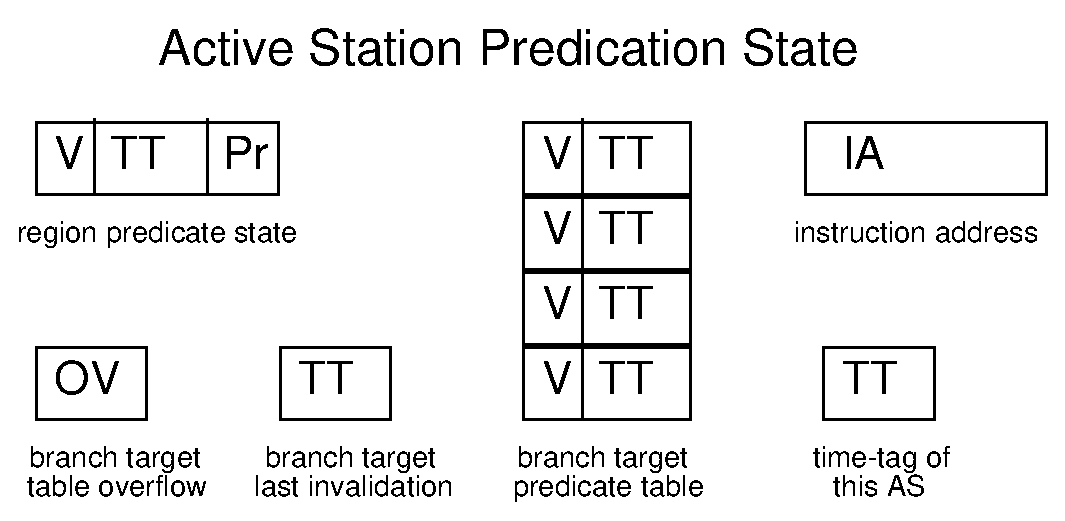
\epsfig{file=state.eps,width=4.0in}
\caption{{\em Active Station Predication State Information.} 
The state within each active station needed for the predication
scheme is shown.
The branch target predicate table is shown with four entries.
Valid bits (V), the region predicate (Pr), an overflow bit (OV),
and time-tag values (TT)
are indicated in the state registers.}
\label{fig:state}
\end{figure}
%
\subsection{Region Predicate State}
%
The first type of state maintained for predicate tracking
is that associated with the
region predicate.  The state associated with the region predicate
has three parts and consists of :
%
\begin{itemize}
\item{a valid bit}
\item{a source time-tag value}
\item{a predicate value}
\end{itemize}   
%
The valid bit is set for all instructions except those instructions
that were dispatched into the execution window following the
taken output path of a conditional branch.  For these latter
instructions, they never associate (nor should they) with the
running regional predicate from the instructions dispatched
into the execution window sequentially before there.
For this reason, the valid bit is turned off when they are
dispatched to ASes.  
It is possible for all other instructions besides
those dispatched following the target of a branch to be enabled
for execution by virtue of them being located in a region that 
might be enabled.  All of these instructions (the greater majority)
are therefor dispatched to ASes with the valid bit set.
Currently, there is no changing of the valid bit after instruction
dispatch.  The source time-tag field of the region predicate
state is that of the AS that last forwarded a region predicate
transaction (more of transactions is described later).
This is identical to the last time-tag value maintained
for input register operands of the AS.  The snarfing condition for
the region predicate is identical as that for register operands and occurs
when the source AS time-tag of a region predicate transaction
is less that the current AS's time-tag but greater or equal to the
last snarfed value.
The last bit of state is the value of the region predicate itself.
A zero value means that the region is disabled, a one value means
that it is enabled.
%
\subsection{Branch Target Predicate State}
%
The second major state maintained by each AS for predication
is a table of branch target predicates.
The table consists of a number of fixed sized entries and
each entry has two parts.
The parts of state for each entry consists of :
%
\begin{itemize}
\item{a valid bit}
\item{a source time-tag value}
\end{itemize}   
%
The valid bit indicates that the entry is used and that
the associated time-tag value is valid.  Any valid entry
indicates that the current instruction is the possible target
of a previous conditional branch and that the current instruction
is therefor currently predicated
to execute (is enabled).  This further means that the output 
region predicate from this instruction should
be set to TRUE.  The exact calculation of the instruction
execution predicate and its output predicate is presented later.
It should be further noted that the time-tag value in a
branch target predicate is effectively the address of the predicate.
The predicate itself (if present in one of these state table entries)
is implicitly TRUE (and therefor enabling) and can be thought of
being sourced from the conditional branch that originated it.
The time-tag value is the address of the AS holding that 
originating conditional branch.

Any number of table entries are possible but the number should
roughly correspond to the number of conditional branches that
are likely to target a single instruction on the average given
the size (in main-line ASes) of any given execution window.
Program characterization can be used to pick a good value for the
number of entries.  When more branch target predicates
are received than there are entries for, an overflow mechanism
is invoked.  Predicate-only active stations are neither assigned
at dispatch time nor are they used in the scheme.
Rather, a dynamic overflow scheme is used to handle these circumstances.
Invalid entries are available for storing
time-tags for new branch target matches to the current instruction.
%
\subsection{Overflow Indication}
%
Next, there is maintained an overflow bit 
for those cases when a given instruction is the
target of more conditional branches than there are branch target
predicate entries in the table just described.
When the overflow bit is clear, it indicates that an overflow
condition is not in effect for the current AS.
If the bit is set, it indicates that an overflow of
branch target predicate matches with the current instruction
address has occurred.  
Since the existence of branch target predicates 
for the current instruction
always indicates
that the current instruction is predicated to execute, no
ambiguity of the predication status is manifested until all existing
branch target predicates are invalidated.
The exact details of the handling of an overflow is discussed later.
%
\subsection{Invalidation Time-Tag State}
%
Finally, each AS can maintain a state register that holds
a time-tag value that can further govern the management of
the branch target predicate table.
This time-tag value is used to prevent the snarfing of
branch target predicate broadcasts that are not applicable to the
current active station.  This state register will be updated
with the latest sourcing AS time-tag value that was associated with 
a branch target predicate invalidation transaction.
This is very analogous to holding the latest time-tag
value snarfed for a register operand but it is applied to
invalidation transactions rather than the more familiar operand
update transactions associated with register and memory operations.
%
\section{General Operation}
%
As instructions execute they forward any significant changes in
predicate information that program ordered future (larger
time-tag valued) instructions will
use to determine their branch domains and whether they are the target of
one or more previous branches.  Three types of predicate forwarding
transactions are identified.  Each of these transactions are
discussed in the following subsections.
A further discussion of the operation follows the introduction
of the various transactions.
%
\subsection{Predicate Related Transactions}
%
Each of the three predicate related transactions
are now discussed in turn.
%
\subsubsection{Region Predicate Transaction}
%
One type of predicate transaction is generated from non-branch instructions.
This predicate transaction type forwards a region predicate value
similar to a register operand update transaction.
When a
non-branch instruction forwards predicate information, it will forward
only a region predicate.  
The following is forwarded in this type of transaction :
%
\begin{itemize}
\item{the sourcing AS time-tag value}
\item{the region predicate value}
\end{itemize}   
%
The snooping ASes in the program ordered future will possibly
snarf this predicate value according to normal snarfing rules for the
comparison of time-tags that are already used for register snarfing.
Note that only those ASes that have their valid bit set in their
region predicate state structure will participate in
region predicate snooping.
Snarfing ASes will update their regional predicate state to reflect the
latest TT value and the new value for the region predicate.  
%
\subsubsection{Branch Target Predicate Transaction}
%
Another type of predicate transaction is generated by conditional branch
instructions.
This type of predicate transaction forwards a 
region predicate value as well as
a branch target predicate.
More information is contained in this type of predicate transaction
as compared with the simpler region predicate transaction already
described.
The fields associated with this transaction include :
%
\begin{itemize}
\item{the sourcing AS time-tag value}
\item{the branch target address}
\item{the output region predicate value}
\item{the output branch target predicate value}
\end{itemize}   
%
Snooping ASes, upon seeing a branch target predicate transaction, 
will snarf and
update its region predicate state the same as if a region predicate 
transaction
(from a
non-branch instruction) was forwarded.
However additional work is
done also.  The snooping AS will compare its instruction address (which
it received at instruction dispatch time)
with the branch target address that is forwarded by the
branch instruction.  If there is a match on the branch target address,
the snooping AS will also look to see if the branch is predicated taken.
If the branch target predicate is true, then that indicates that
instruction flow is currently predicted to come through the taken
path.  
In this circumstance, the snarfing AS will allocate
a previously unused branch target predicate state register for holding
the TT value of the originating AS with the conditional branch.
%
\subsubsection{Branch Target Invalidation Transaction}
%
Each branch target predicate transaction can be used by at most only
one instruction located in the program ordered future of the
conditional branch that originated the transaction.
A means is needed to ensure that only one instruction (the true
target of the conditional branch) makes use of a branch target
predicate transaction.
More than one instruction in the program ordered future from
the conditional branch may match on the branch target address.
This can occur when (for example) the target of a branch is
located within a loop in the program code.
Since several instructions (for example, one from each iteration of a loop) 
can have the same instruction
address, some means needs to be provided to distinguish the
first of these (in program ordered time) from the remaining (subsequent) ones.
This situation is handled by an AS holding the instruction that
is the 
target of a conditional branch.  
This AS may be either the actual target of the branch (the first
matching one after the conditional branch) or a subsequent instruction.
In either case the same action is taken.
Such an AS will forward a special type of
transaction that will invalidate the previous branch target
predicate transaction that had already been previously forwarded.
This special transaction consists of the following fields :
%
\begin{itemize}
\item{the sourcing AS time-tag value}
\item{the branch target instruction address}
\item{the time-tag of a branch target predicate that is to be invalidated}
\end{itemize}   
%
The sourcing AS time-tag value is used in the snooping
determination as is typical with other (register and memory) transactions.
The branch target address is also used to see if it matches with
the instruction address in the snooping AS.
When a match is determined,
a search is made in the branch target
predicate table for a matching time-tag for the AS holding the original
conditional branch.  This latter search can actually occur in parallel
with the branch target comparison but that is an implementation issue.
If an entry is found, it is deleted (marked as
invalid) and that
entry is available for reuse.  Also, if an entry is found, the time-tag
state register that holds the last invalidation time-tag value,
maintained within the AS, is updated to reflect the
sourcing AS's time-tag value.  This invalidation time-tag
value can be used to avoid false branch target predicate matches
in the future.  Once an invalidation time-tag value is
acquired, future branch target predicate transactions would
need to be sourced from an AS with a time-tag value that is
at least as large as the invalidation time-tag value.
This use is correctly forcing an AS to avoid accepting
branch target predicates that actually belong to the correct target of
the branch.
This feature is not strictly needed, as the whole scheme will
work properly without maintaining this invalidation
time-tag state, but it serves to reduce some unnecessary flipping
of the enabling execution predicate for false 
branch target matching instructions.
%
\subsection{Detailed Operation}
%
Given a regional predicate (Pr),
the execution predicate (Pe) of the AS, its enabling predicate,
is computed as :
\[
	Pe = Pr,input + (\mbox{any branch target predicates})
\]
Similarly, a new output region predicate (Pr) 
for a non-conditional branch instruction 
is computed 
by the snarfing AS as follows :
\[
	Pr,output = Pr,input + (\mbox{any branch target predicates})
\]
If the output region predicate changes from its previous value, it is
forwarded as expected.  
As expected, the output predicates from branch instructions are
computed according to :
\[
	Pr,output = Pe * (\mbox{branch predicted not-taken})
\]
and
\[
	Pt,output = Pe * (\mbox{branch predicted taken})
\]
The first of these is the output regional predicate (also the
output predicate for the not-taken output path from the branch).
The second is the Branch Target Predicate (Pt) and is for the 
target of the branch.  Both output
predicate values are forwarded using a Branch Target Predicate
transaction as previously discussed.

The use of forwarding the branch target instruction address rather than
the target time-tag value (previously proposed some time ago) is to handle
the situation where the target of a branch does not lie the same number
of ASes forward in program ordered 
time as the branch target address might indicate.  
A dynamic change in the instruction flow (instructions dispatched following
the taken output path of a branch) may have been dispatched into the
execution window and this can obviously cause target instructions of a
conditional branch to lie any number of ASes into program ordered
future, rendering
the relative computation of a target TT value to be of no use.  Rather,
by having conditional branch instructions 
broadcast the absolute target instruction
address, the possible target instruction can snarf on an instruction
address match regardless of how many ASes into program ordered future 
it may lie
within the execution window.

When a branch instruction computes a change in its output branch
target predicate such that it becomes false (the branch is no longer
predicated to be taken or it is no longer predicted to execute itself),
it will perform a predicate forward operation.  Snooping ASes will
again match on the target address but will also search to see if that
branch target predicate from the originating branch instruction was
previously recorded.  If it was previously recorded, the branch target
predicate address state register entry that was occupied becomes
unoccupied.  This amounts to the loss of an enabling input to its
execution predicate computation and its output region predicate value.  
If the
output predicate region value changes, this instruction will perform,
in turn, its own predicate forward operation.
Of course, the target of a branch instruction can itself be a branch
instruction and this is handled in the expected straight forward manner
(as in the current scheme also).  

No ordering of any kind is
needed for the forwarding of predicate transactions, whether it be from
a non-branch instruction or from a branch instruction.  This latter
feature is a critically important one 
because current predicate forwarding bus mechanisms, when
combined with the existing grouping of ASes into Sharing Groups, cannot
necessarily guarantee the order of predicate forward operations.  The
order of predicate forward operations may be mixed up due to additional
structural hazards in the machine such as the priority and queue delay
for the use of a Processing Element when one may be needed for the
execution of a branch that may require some non-trivial computation.
In any event, it is certainly advantageous to not require a strict
real-time ordering of predicate forward operations.

A difficulty with the proposed scheme occurs when the target of a
branch already has all of its architected (machine configured) branch
target predicate address state registers used and then a
match occurs with a new originating branch instruction that was not
previously recorded in the AS.  What we would like to do is to allocate
an additional predicate address state register to hold the new
predicate source TT value but this is not possible since all of the
registers are used up.  Rather we can either ignore the new branch
match condition or we can replace an existing branch predicate address
with the new one.  In either case, the overflow bit is set in the AS
state.  The replacement policy for handling overflow branch target
matches is something that could be researched further 
to find the policy
that gives best execution performance.  
We have to set the overflow bit
because we need to track that an overflow occurred.  
This is necessary so that after all existing branch target 
predicates become false,
due to subsequent forward operations,
and when the region predicate of the current AS also goes false, we need
to know that there is still an ambiguity about whether the current AS
is predicated to execute or not.  The problem comes into play on how to
resolve this ambiguity.  The most natural mechanism would require the
addition of a predicate backwarding bus of some sort in order for
ASes that have reached an ambiguous state to make a request backwards.
This backwards request would essentially ask all branch instructions
to resend a predicate forwarding transaction so that any branch target
matches for those branches that are predicated to execute, and to
execute taken, can be be snarfed by the ambiguous AS.  At least
one backwarding request would have to be made for any AS in an
ambiguous state before the ambiguous AS could be allowed to commit.
Another strategy for resolving ambiguous ASes besides requiring
a backwarding bus may be to design some way to just signal
the ASes holding conditional branches to initiate branch target
predicate transactions.  This would also provide the necessary
disambiguating transactions that would be needed.
%
\section{Branch Target Predicate Table Entry Replacement Policies}
%
Some thought can now be given to the replacement policy for storing
matching branch target predicate addresses.  We obviously would want to
minimize the likelihood of having as AS ever reaching an ambiguous
state.  The likelihood of an AS reaching an ambiguous state is already
probably quite low but will always remain non-zero if the number of
configured branch target predicate address storage registers in an AS
is less than the AS window size (same as the current scheme).  The
likelihood of an AS reaching an ambiguous state will only occur after
both overflow occurs and when its region predicate goes false.  
This is somewhat less than the probability of some number of preceding
branches all predicting that they are both being executed and are
also being predicted as taken, and when 
all of those branches target a single AS.  
This may indeed be a very small probability.
Simulations can show the exact likelihoods
involved with actual benchmark programs codes.  
Replacement policies that have been thought
of include :
%
\begin{itemize}
\item{ignore the latest match and keep existing entries}
\item{replace a branch target predicate address such that
the latest time-tag values are retained}
\item{replace a branch target predicate address such that
the earliest time-tag values are retained}
\item{maintain an age associated with a branch target predicate address
(updated each clock for example) and only replace the oldest aged
entry}
\item{maintain an age and replace the youngest aged entry}
\item{some combination of the above}
\end{itemize}   
%
As already stated, simulations could explore which replacement policy
might perform best.
%
\section{Other Possibilities}
%
Some other manipulations of these dynamic predicates maintained by an
AS may be possible and may or may not provide some performance
advantages.  Currently, region predicates are maintained dynamically by
a chain of regional predicate dependencies.  State contained in an
AS, to maintain this chaining, primarily consists of 
a region predicate address and a region
predicate value.  If a target of a branch is serving as the previous
link in a region predicate chain for a future instruction and that
branch target AS snarfs a branch predicate forward operation such that
its execution predicate now only depends on its own region predicate,
that branch target AS can forward information to succeeding ASes so
that they can unlink the branch target address and revert back to the
region predicate address that was the original region predicate of the
branch target AS.  This unlinking operation would be accomplished by the
branch target AS forwarding its own region predicate address along with
its own predicate forward operation.  
This would be a \textit{GOTO-predicate-address}
for future ASes that could be used to essentially unlink the
intermediate branch target AS.  The snarfing AS of a predicate forward
operation with a GOTO predicate address could then update its
own predicate address to that of the GOTO value rather than the
existing value (that of the AS that was the target itself of a
branch).  

What would a region predicate unlink operation do to help overall
operation ?  It will eliminate one indirection for those ASes that were
dependent on an AS that was itself the target of a branch when that AS's
execution predication no longer is valid through the taking of any
branches.  Of course, this unlinking operation can continue backwards
through many combinations of ASes that are the target of a branch.
Other unlinking operations are also possible but do not appear do be as
useful as the one described so far since they would quickly degenerate,
into likely forming additional chaining links 
(often the same as before) as the
intermediate instructions send their own predicate updates forward.
As already stated, it is not intuitive how much performance may
be gained from these additional (and increasingly esoteric)
techniques but these possibilities are mentioned for completeness.
%
\section{Conclusions}
%
We have presented the overview of a new predication scheme.
This new scheme is performed dynamically as instructions
execute and requires no predication of instructions before they
are dispatched the execution window. 
The use of a centralized predication tracking buffer is entirely
avoided.
And finally, and importantly, the scheme scales since it
doesn't depend on either a centralized microarchitectural resource
or any buses that need to span the whole length of the machine.
%
%
%
\bibliographystyle{latex8}
\bibliography{pred}
\end{document}
%
%
